\documentclass[
    twoside=false,
    twocolumn=true,
    fontsize=11pt,
]{scrarticle}
\usepackage{xcolor}
\definecolor{seeblau}{HTML}{00A9E0}
\definecolor{seegrau}{HTML}{9AA0A7}

\definecolor{seeblau1}{HTML}{CCEEF9}
\definecolor{seeblau2}{HTML}{A6E1F4}
\definecolor{seeblau3}{HTML}{59C7EB}
\definecolor{seeblau4}{HTML}{00A9E0}
\definecolor{seeblau5}{HTML}{008ECE}


\usepackage{graphicx}
\usepackage{amsmath}
\usepackage{subcaption}
\usepackage{wrapfig}
\usepackage[english]{babel}
\usepackage{blindtext}
\usepackage{microtype}
\usepackage{siunitx}
\usepackage[utf8]{inputenc}
\usepackage{csquotes}
\usepackage{nicefrac}
\usepackage[T1]{fontenc}
\usepackage{amsfonts}
\usepackage{amssymb}
\usepackage{tikz}

\usepackage{siunitx}

\usepackage{libertinus, libertinust1math}
\usepackage{roboto}

\setkomafont{disposition}{\normalfont\sffamily}


% not recommended with KOMA-script
% make table of contents sans-serif
% \usepackage{tocloft}
% \renewcommand\cftchappagefont{\normalfont}
% \renewcommand\cftchapfont{\normalfont}
% \renewcommand\cftchappresnum{\bfseries}
% \renewcommand\cftchapaftersnum{}
% \renewcommand{\cftchapfont}{\sffamily}
% \renewcommand{\cftsecfont}{\sffamily}
% \renewcommand{\cftsubsecfont}{\sffamily}
% \renewcommand{\cftchappagefont}{\sffamily}
% \renewcommand{\cftsecpagefont}{\sffamily}
% \renewcommand{\cftsubsecpagefont}{\sffamily}

% caption
\usepackage{caption}
\captionsetup{
	% font={sf},
	labelfont={sf, bf, color=seeblau},
	labelsep=quad,
	labelformat=simple,
}

% links
\usepackage{hyperref}
\hypersetup{
	colorlinks=true,
	linkcolor=seeblau,
	citecolor=seeblau,
	urlcolor=seeblau,
	% hidelinks=true
}

% bibliography
\usepackage[
	style=numeric-comp, % comp = compressed 4,5,6,7 -> 4-7
	sorting=none,		% Sort by appearance
	% autocite = superscript,
	% backref=true,
	hyperref=true,
	url=true,
	maxbibnames=100
]{biblatex}
\DefineBibliographyStrings{english}{%
    backrefpage  = {see p.}, % for single page number
    backrefpages = {see pp.} % for multiple page numbers
}

% remove issue
\AtEveryBibitem{%
  \clearfield{number}
}

\usepackage{float}
% \floatplacement{figure}{h}
% \floatplacement{table}{H}

% loosen float placement rules
\renewcommand{\topfraction}{0.8}
\renewcommand{\bottomfraction}{.8}
\renewcommand{\textfraction}{0.1}
\renewcommand{\floatpagefraction}{.9}
% make floats less likely to be placed on a separate page
\setcounter{totalnumber}{9}
\setcounter{topnumber}{9}
\setcounter{bottomnumber}{9}

% decrease space between floats and text
\setlength{\textfloatsep}{0.5cm}
\setlength{\floatsep}{0.5cm}


\usepackage{adjustbox}

\usepackage{datetime}
\newdateformat{dotdate}{
	\twodigit{\THEDAY}.\twodigit{\THEMONTH}.\THEYEAR
}
\newdateformat{monthyeardate}{%
  \monthname[\THEMONTH] \THEYEAR}


% header and footer
\usepackage[
  markcase=noupper
]{scrlayer-scrpage}% activates pagestyle scrheadings automatically
\clearpairofpagestyles
\setkomafont{pageheadfoot}{\normalfont\sffamily}
\setkomafont{pagenumber}{\normalfont\sffamily}
% \chead*{\color{seegrau} Draft \dotdate\today}
\ofoot*{\pagemark}
\ohead*{\rightmark}


\usepackage{ifthen}
\newcommand{\markieren}[4]{
    \ifthenelse{\equal{#1}{}}{}{\adjustbox{padding=3pt, bgcolor=seeblau1, margin=-1pt}{\strut{\sffamily\robotoMedium{#1}}}\\}
    \ifthenelse{\equal{#2}{}}{}{\adjustbox{padding=3pt, bgcolor=seeblau2, margin=-1pt}{\strut{\sffamily\robotoMedium{#2}}}\\}
	\ifthenelse{\equal{#3}{}}{}{\adjustbox{padding=3pt, bgcolor=seeblau3, margin=-1pt}{\strut{\sffamily\robotoMedium{#3}}}\\}
	\ifthenelse{\equal{#4}{}}{}{\adjustbox{padding=3pt, bgcolor=seeblau4, margin=-1pt}{\strut{\sffamily\robotoMedium{#4}}}}
}

\addbibresource{literature.bib}

\begin{document}

\title{title}
\subtitle{subtitle}
\author{Aurel Müller-Schoenau, Leon Oleschko}
\date{\dotdate\today}


% make a custom title page
\begin{titlepage}
    \sffamily
    \vspace*{3cm}
    {
        \fontsize{32}{32}
        \markieren{}{Evanescent light scattering}{Optical Tweezers}{Random Walk}
    }
    \vspace{.25cm}\\
    {
        \Large
        Aurel Müller-Schoenau, Leon Oleschko\\
        Supervised by Krishna Kumar, Karthika
        \vspace{.05cm}\\
        13.11.2024
        \vspace{.25cm}\\
        \normalsize
        Physikalisches Fortgeschrittenenpraktikum 2\\
        Universität Konstanz
    }
    \vfill
    {
        \normalfont\normalsize
        Abstract auf Englisch (10-15 Zeilen)
        \blindtext[2]
    }
    \vfill
    \begin{flushright}
        Available at \url{www.github.com/leoole100/fp2}.
    \end{flushright}
\end{titlepage}

\section{Introduction}
Using the statistics of the random walk small forces can be measured.
This is demonstrated on colloidal particles in an aqueous solution.
Forces are applied using optical tweezers and the position is measured with different microscopy techniques.


% \subsection{Physical Principles}
% kompakten Zusammenstellung der physikalischen Grundlagen


\section{Methods}
\begin{figure}
    \centering
    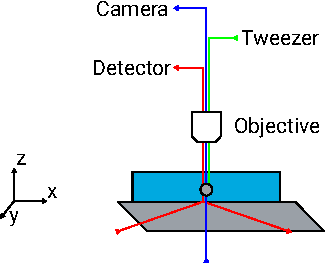
\includegraphics{figures/setup.pdf}
    \caption{Schematic of the experimental setup. Optical tweezers in green, transmission light microscopy in blue and total internal reflection microscopy in red.}
    \label{fig:setup}
\end{figure}
This experiment operates with light on small particles (in the range of \SI{1}{\micro m} \cite{instructions}) in an aqueous solution.
This is shown in \autoref{fig:setup} as the gray circle in the blue box. 

Using an optical tweezers setup the particle can be trapped in the center of the sample.
This results in a 3-dimensional harmonic potential, with a spring constant that is roughly proportional to the trap strength.

To directly observe the particle transmission light microscopy is used.
For this a blue led is used to illuminate the particle from below.
This allows the particle position to measured in $x$ and $y$ direction.

To measure the position in $z$ direction, total internal reflection microscopy is used.
For this a red laser is totally reflected at the boundary below the aqueous solution to create an evanescent wave.
This wave scatters off the particle into a sensitive photo detector.

% \section{Procedure}

\section{Results}
All recorded data and the analysis is available at \url{www.github.com/leoole100/fp2}.

\subsection{Transmission Light Microscopy}
\begin{figure}
    \centering
    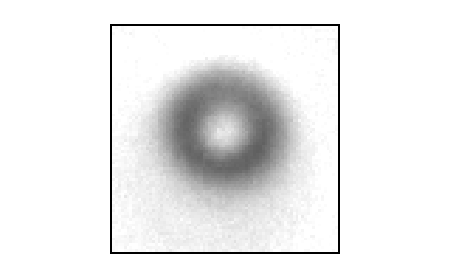
\includegraphics{figures/01_01_1_particle.pdf}
    \caption{Transmission light microscopy of a observed particle. The radius of the particle is \SI{14(2)}{px}, equivalent to \SI{1.86(27)}{\micro m}.}
    \label{fig:01particle}
\end{figure}
In the first section of the experiment, the particles were observed using a transmission light microscope setup.
For this images with a resolution of $600\times 800$\si{px} were recorded with a frequency of \SI{10}{Hz} for \SI{10}{min}.
The magnification of the microscope was assumed to be \SI{0.13319672}{\micro m/px} \cite{instructions}, this is the main systematic error of this measurement procedure.

The images were normalized with a black (illumination off) and white (illumination on, particle not in frame) reference image, to remove the influence of dust in the imaging elements.
The particle that was used for this experiment is shown in \autoref{fig:01particle}, after the normalization.

\begin{figure*}
    \centering
    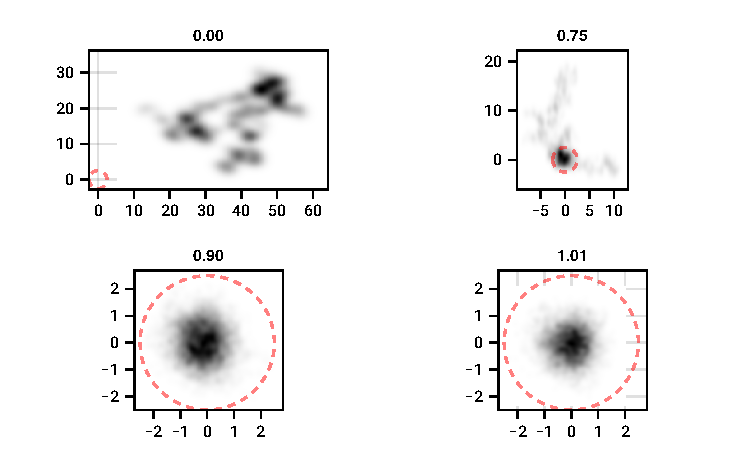
\includegraphics{figures/01_03_1_bivariate.pdf}
    \caption{Density of recorded particle positions, grouped by optical trap stiffness. The red circle indicates the approximate radius of the optical trap \SI{2.5}{\micro m}.}
    \label{fig:01bivariate}
\end{figure*}
To determine the trajectory of the particle, an effective center of mass was calculated for each frame:
\begin{equation}
    \vec{r}(t) = \iint \vec{r} \cdot \left(1-I(\vec{r}, t)\right)^2 d\vec{r}    
\end{equation}
The density of the resulting trajectory is shown in \autoref{fig:01bivariate} for different optical trap stiffnesses.
The approximate radius of the optical trap of \SI{2.5}{\micro m} is drawn as a red circle.
For the trap stiffness of \SI{0}{}, the particle is free to wander around, for the higher stiffnesses like \SI{1.01}{} the particle is mostly confined to the trap.\\
For a weak trap like \SI{0.75}{} the particle is still mostly confined to the trap, but can escape the linear trap region and randomly wander around. 
This happened multiple times during the shown measurement.

\begin{figure}
    \centering
    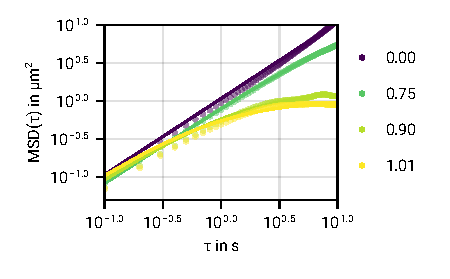
\includegraphics{figures/01_02_2_msd.pdf}
    \caption{Mean Square Displacement for different optical trap stiffnesses, fit: \autoref{eq:01_mdl_msd}}
    \label{fig:01msd}
\end{figure}
\subsection*{Mean Square Displacement}
A method to describe the trajectory of a random walk is the mean square displacement (MSD) \cite{wiki:msd}.
This is defined as the average of the squared distance of the particle from the starting point \cite{wiki:msd}:
\begin{equation}
    \text{MSD}(t) = \frac{1}{N} \sum_i^N \left( x_i\left(t\right) - x_i\left(0\right) \right)^2 
\end{equation}
Here a different implementation using the autocorrelation of the velocity was used, to achieve a more stable result.
This was implemented by \cite{jl:msd}.
The resulting MSD for different optical trap stiffnesses is shown in \autoref{fig:01msd}.

The MSD can be described by the following model:
\begin{equation}
    \text{MSD}(\tau) = \frac{1}{\frac{1}{D_0 \tau} + \frac{1}{\text{MSD}(\infty)}}
    \label{eq:01_mdl_msd} 
\end{equation}

For a free particle the $\text{MSD}(\infty)=\infty$ and the MSD grows linearly with $D_0$ over time \cite{wiki:msd,instructions}.\\
The diffusion Coefficient $D_0$ estimated using the fit in \autoref{tab:01spring} is equivalent to the theoretical value of $D_0 = \frac{k_B T}{6 \pi \eta r} = \SI{0.122(18)}{\micro m ^2 / s}$ \cite{instructions}, with $r = \SI{1.86(27)}{\micro m}$ and $\eta = \SI{0.955}{mPa\cdot s}$\cite{n:water}.
The error in the magnification of the microscope does increase the uncertainty.

For a confined particle the MSD reaches a plateau at $\text{MSD}(\infty)$ \cite{instructions}.
This happens for the higher trap stiffness (\SI{0.90}{}, \SI{1.01}{}) and the estimated values $k_{\text{MSD}(\infty)} = \frac{2 k_B T}{\text{MSD}(\infty)}$ are shown in  \autoref{tab:01spring} and \autoref{fig:01spring}.\\
For the lower measured spring stiffness (\SI{0.75}{}), the MSD does not reach a plateau, as it partially escapes the trap and wanders around (see \autoref{fig:01bivariate}).
Therefore this procedure is not adequate for such low spring stiffnesses.

\begin{table}
    \centering
    \begin{tabular}{r|l|l|l}
        Stiffness & $D_0$ in \SI{}{\micro m^2/s}& $k_{\text{MSD}(\infty)}$ & $k_V$ \\
        \hline        
        \SI{0}{}    & \SI{0.10728(93)}{}    & NA                & \SI{0}{} \\
        \SI{0.75}{} & \SI{0.07793(03)}{}    & NA                & \SI{0.9011(45)}{}\\
        \SI{0.90}{} & \SI{0.0678(24)}{}     & \SI{6.471(62)}{}  & \SI{4.7177(62)}{}\\
        \SI{1.01}{} & \SI{0.05384(08)}{}    & \SI{8.968(23)}{}  & \SI{6.021(12)}{}\\
    \end{tabular}
    \caption{Estimated diffusion constant and spring constant in \SI{}{\nano N / m}.}
    \label{tab:01spring}
\end{table}
\subsubsection*{Potential}
A more detailed analysis can be done by looking at the distribution of the particle positions.
For this the probability density function (PDF) of the particle positions has to be estimated.
This is done using kernel density estimation (KDE) with a Gaussian kernel \cite{jl:kde}.
The resulting 2-dimensional PDF is shown in \autoref{fig:01bivariate}.\\
As the density is small for large parts of the explored 2d space, the data is reduced by aggregating along the image coordinates $x$ and $y$.
As the Potential should by rotationally symmetric, the data from the $x$ and $y$ axis should not significantly deviate.

\begin{figure}
    \centering
    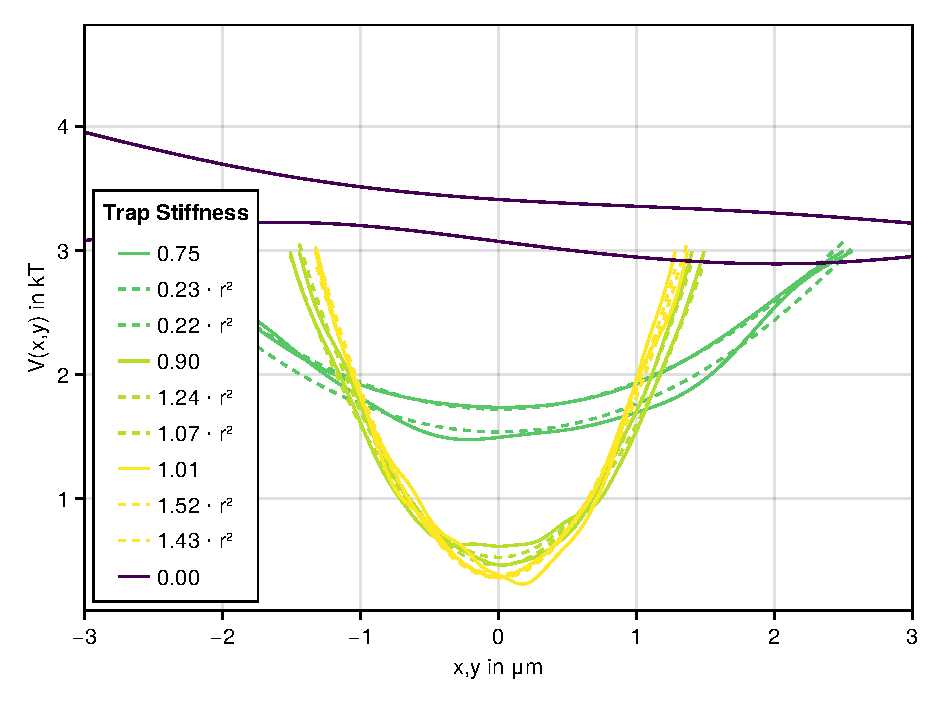
\includegraphics{figures/01_03_3_axis.pdf}
    \caption{Measured Potential, with quadratic fit.}
    \label{fig:01potential}
\end{figure}
\begin{figure}
    \centering
    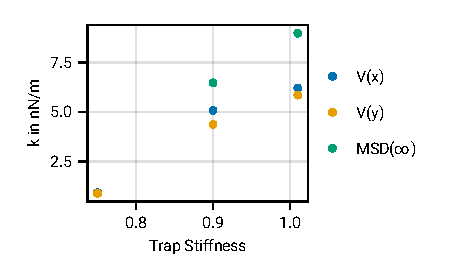
\includegraphics{figures/01_03_4_spring_constants.pdf}
    \caption{Differently measured spring constants.}
    \label{fig:01spring}
\end{figure}
Using the Maxwell Boltzmann relations \cite{instructions}, the potential at a position $p$ can be calculated from the PDF:
\begin{equation}
    V(p) = - \frac{\log{\text{PDF}(p)}}{k_B T}
\end{equation}
The resulting potential is shown in \autoref{fig:01potential}.
The parts of the measurements with a $\text{PDF}(x)>0.05$ are used for a quadratic fit, to estimate the spring constant.
The resulting spring constants are shown in \autoref{fig:01spring} and \autoref{tab:01spring} and are in the same order of magnitude. 

For the lower spring constant of \SI{0.75}{}, the potential begins quadratically, but flattens after approximately \SI{2.5}{\micro m}.
This is due to the limited size of the trap, but the spring constant can still be estimated.

This method allows for the measurement of a spring constant as low as \SI{0.9011(45)}{\nano N /m}, which means over the used length scales that forces in the order of \SI{1}{\femto N} can be measured.

\subsection{Total Internal Reflection Microscopy}
\textit{Note:} As some references in \cite{instructions} led to nowhere, we implemented our own methods.\\
To measure the particle movement in the vertical direction, \textit{Total Internal Reflection Microscopy} was used: A laser beam is totally reflected at the glass-water boundary below the particle. The resulting evanescent field decays exponentially in the $z$ direction, which means the intensity of the light scattered by the particle allows for precise position measurement on the vertical axis.


\subsubsection*{Position and Diffusion Coefficient}
\begin{figure*}
    \centering
    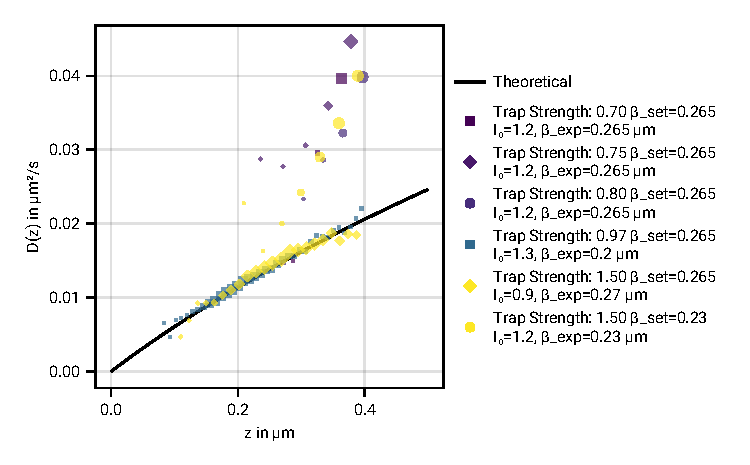
\includegraphics{figures/02_04_01_diffusion.pdf}
    \caption{Estimated diffusion coefficient for different measurements. For differently set evanescent wave parameters $\beta$ in \SI{}{\micro m}. If it is shown for a different $\beta$, it is noted in brackets.}
\end{figure*}

The $z$ distance between particle and wall can be calculated using the formula \cite{instructions}
\begin{equation}
 \label{eq:calculate_z}
 z = \frac{\log(I) - \log(I_0)}{-\beta}
\end{equation}
where $I$ is the scattered light intensity and $I_0$ is the maximum possible intensity, i.e. $z=0$, when the particle touches the glass surface. $\beta^{-1}$ is the characteristic length of the evanescent field.\\
The $z$-dependent diffusion coefficient can be calculated from the position changes $\Delta z$ in a given $z$ interval. For Brownian motion these should be normally distributed with
\begin{equation}
\label{eq:D_delta_t}
 \sigma^2 = 2 \cdot D \cdot \Delta t
\end{equation}
where $D$ is the diffusion coefficient \cite{instructions}. In reality there is an additional component owing to measurement uncertainty which does not depend on $\Delta t$. To eliminate it, the derivative with respect to $\Delta t$ is estimated by calculating \autoref{eq:D_delta_t} for different $\Delta t$, followed by a linear regression.\\
Close to a wall, the diffusion coefficient can be modeled \cite{instructions} by the equation
\begin{equation}
 \label{eq:D_Brenner_approx}
 D_\bot = \frac{D_0}{\left(\frac{R}{z}\right) + 0.2 \log\left(\frac{R}{z}\right) + 0.9712}
\end{equation}
with the radius $R$ of the particle and the free diffusion coefficient $D_0$ given by \cite{instructions}
\begin{equation}
 \label{eq:D_0}
 D_0 = \frac{k_B T}{6 \pi \eta R}
\end{equation}
The radius $R$ is known from the first part of the experiment.


\begin{figure*}
    \centering
    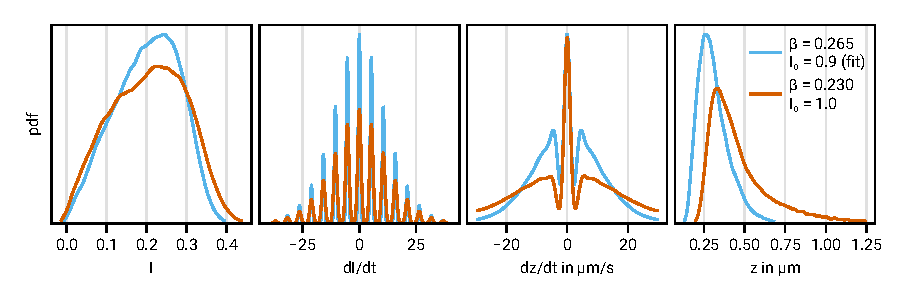
\includegraphics{figures/02_04_02_hist.pdf}
    \caption{Distribution of measurements for the same trap stiffness \SI{1.5}{} with different $\beta$.}
\end{figure*}

\subsubsection*{Potential}
\begin{figure}
    \centering
    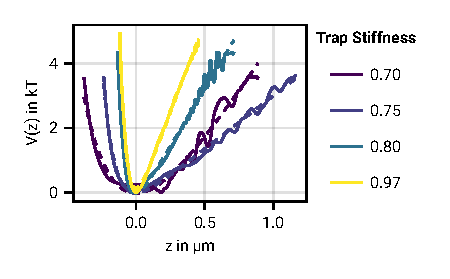
\includegraphics{figures/02_05_01_potential.pdf}
    \caption{Measured Potential for different optical trap stiffnesses.}
\end{figure}
\begin{figure}
    \centering
    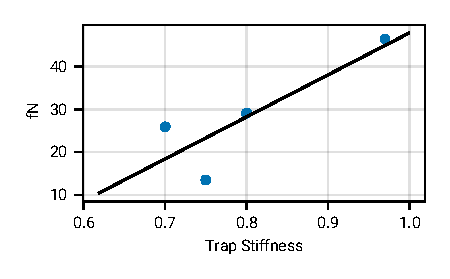
\includegraphics{figures/02_05_02_gravity.pdf}
    \caption{Linear fit from Potential.}
\end{figure}
\begin{figure}
    \centering
    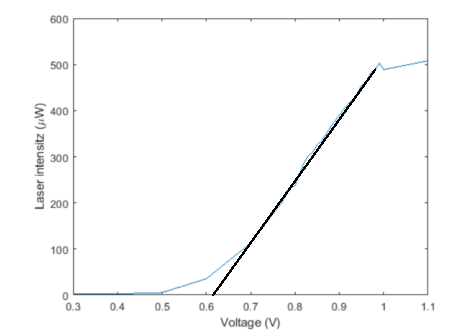
\includegraphics{figures/laser_linearity.pdf}
    \caption{Relation of the trap stiffness variable to the actual power.}
\end{figure}
\begin{figure}
    \centering
    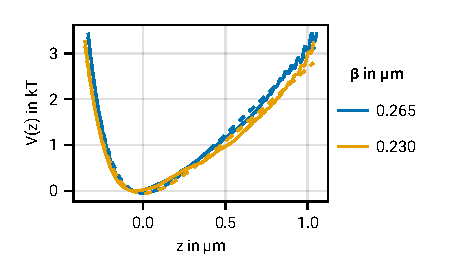
\includegraphics{figures/02_06_01_different_beta.pdf}
    \caption{Measured potential at same trap stiffness, but different illumination angle.}
\end{figure}
\begin{table}
    \centering
    \begin{tabular}{r|l|l}
        stiffness   & effective gravity in \SI{}{\femto N}  & $\kappa^{-1}$ in \SI{}{\nano m} \\
        \hline
        0.70  & \SI{25.88(55)}{} & \SI{260.4(84)}{}\\
        0.75  & \SI{13.47(61)}{} & \SI{ 84.2(12)}{}\\
        0.80  & \SI{29.06(18)}{} & \SI{47.28(83)}{}\\
        0.97  & \SI{46.38(11)}{} & \SI{ 45.6(26)}{}
    \end{tabular}
    \caption{Fit Parameters from the potential. }
\end{table}



\section{Discussion}

\addcontentsline{toc}{section}{Literature}
\nocite{*}
\printbibliography

\end{document}
